\documentclass[12pt]{article}

\usepackage{mathtools}

% \usepackage[margin=1in]{geometry}

\newcommand*{\eu}{e}
\newcommand*{\iu}{i}

\DeclarePairedDelimiter{\bra}{\langle}{\rvert}
\DeclarePairedDelimiter{\ket}{\lvert}{\rangle}
\DeclarePairedDelimiterX{\braket}[2]{\langle}{\rangle}
  {#1\,\delimsize\vert\,\mathopen{}#2}

\usepackage{biblatex}
\addbibresource{report.bib}

\usepackage[hidelinks]{hyperref}

\title{Solving the Transverse-Field Ising Model on a Quantum Computer}
\author{David Basoco \and Jack Hetherington \and Davis Rash \and Tim Ross}
\date{October 4, 2023}

\begin{document}
  \maketitle


  \section{Introduction}

  The transverse-field Ising model is a quantum mechanical model of a spin lattice. In one dimension, the model can be described by the Hamiltonian
  \begin{equation}
    \label{eq:hamiltonian}
    H = \sum_{i = 1}^{n} \sigma_{i}^{x} \sigma_{i + 1}^{x}
        + \sigma_{1}^{y} \sigma_{2}^{z} \dotsm \sigma_{n - 1}^{z} \sigma_{n}^{y}
        + \lambda \sum_{i = 1}^{n} \sigma_{i}^{z},
  \end{equation}
  where \( \lambda \) is the transverse magnetic field strength. The second term maps periodic boundary conditions to fermionic degrees of freedom. Its effect vanishes for \( n \to \infty \) but has finite effects.

  We solve the transverse-field Ising chain exactly for \( n = 4 \) sites on the \texttt{ibm\_nairobi} 7-qubit quantum computer and compare our results to the original findings~\cite{CerveraLierta18}.


  \section{Quantum Gate Operations}

  To solve the Ising model on a quantum computer, we need to diagonalize Eq.~\eqref{eq:hamiltonian}. We do this by applying a unitary disentangling operator \( U_{\textnormal{dis}} \) such that
  \begin{equation}
    \tilde{H}
      = U_{\textnormal{dis}}^{\dagger} H
        U_{\textnormal{dis}}^{\vphantom{\dagger}},
  \end{equation}
  where \( \tilde{H} \) is a noninteracting Hamiltonian. For the Ising model, the method to obtain the \( U_{\textnormal{dis}} \) is threefold.
  \begin{enumerate}
   \item We first need to map spins to fermionic modes with the Jordan--Wigner transform.
   \item Then we need to get the fermions in moment space by applying the Quantum Fourier transform.
   \item Finally, we perform the Bogoliubov transform to decouple the modes in opposite momenta.
  \end{enumerate}
  This gives us the three-step recipe for our unitary disentangling operator
  \begin{equation}
    U_{\textnormal{dis}}
      = U_{\textnormal{JW}} U_{\textnormal{FT}} U_{\textnormal{Bog}}.
  \end{equation}


  \subsection{Jordan--Wigner Transformation}

  Under the Jodan--Wigner transformation
  \begin{align}
    \label{eq:jordan-wigner}
    c_{j}
      &= \biggl( \prod_{l < j} \sigma_{l}^{z} \biggr)
         \frac{\sigma_{j}^{x} - \iu \sigma_{j}^{y}}{2},
    &
    c_{j}^{\dagger}
      &= \frac{\sigma^{x}_{j} - \iu \sigma^{y}_{j}}{2}
         \biggl( \prod_{l < j} \sigma^{z}_{l} \biggr),
  \end{align}
  the Hamiltonian becomes
  \begin{equation}
    \label{eq:hamiltonian-fermion}
    H_{c}
      = \frac{1}{2}
        \sum_{i = 1}^{n} (c_{i + 1}^{\dagger} c_{i}^{\vphantom{\dagger}}
                          + c_{i}^{\dagger} c_{i + 1}^{\vphantom{\dagger}}
                          + c_{i}^{\dagger} c_{i + 1}^{\dagger}
                          + c_{i}^{\vphantom{\dagger}}
                            c_{i + 1}^{\vphantom{\dagger}})
        + \lambda \sum_{i = 1}^{n} c_{i}^{\dagger} c_{i}^{\vphantom{\dagger}}.
  \end{equation}
  Fortunately, the Jordan--Wigner transformation requires no gates to implement; it is a simple relabeling of the qubits.


  \subsection{Fourier Transformation}

  Now we need to get the fermionic modes to momentum space with the quantum Fourier Transform
  \begin{equation}
    \label{eq:qft}
    b_{k}
      = \frac{1}{\sqrt{n}}
        \sum_{j = 1}^{n} \eu^{2 \pi \iu j k / n} c_{j}, \qquad
    k = -\frac{n}{2} + 1, \dotsc, \frac{n}{2}
  \end{equation}
  Although this is valid in general, we have \( n = 2^{m} \), permitting us to use the fast Fourier transform. The resulting Hamiltonian is
  \begin{equation}
    H_{b}
      = \sum_{k = -n / 2 + 1}^{n / 2}
        \biggl[
          2 \biggl( \lambda - \cos \frac{2 \pi k}{n} \biggr)
          b_{k}^{\dagger} b_{k}^{\vphantom{\dagger}}
          + \iu \sin \biggl( \frac{2 \pi k}{n} \biggr)
            (b_{-k}^{\dagger} b_{k}^{\dagger}
             - b_{-k}^{\vphantom{\dagger}} b_{k}^{\vphantom{\dagger}})
        \biggr].
  \end{equation}


  \subsection{Bogoliubov Transformation}

  The final step is to decouple the modes that have opposite momenta using the Bogoliubov transformation
  \begin{subequations}
    \begin{align}
      a_{k}
        &= u_{k}^{\vphantom{\dagger}} b_{k}^{\vphantom{\dagger}}
           + \iu v_{k}^{\vphantom{\dagger}} b_{-k}^{\dagger}, \\
      a_{k}^{\dagger}
        &= u_{k}^{\vphantom{\dagger}} b_{k}^{\dagger}
           + \iu v_{k}^{\vphantom{\dagger}} b_{-k}^{\vphantom{\dagger}},
    \end{align}
  \end{subequations}
  which corresponds to a matrix equation with the solution
  \begin{equation}
    B_{k}^{n}
      = \begin{pmatrix}
              \cos(\theta_{k} / 2) & 0 & 0 & \iu \sin(\theta_{k} / 2) \\
                                 0 & 1 & 0 &                        0 \\
                                 0 & 0 & 1 &                        0 \\
          \iu \sin(\theta_{k} / 2) & 0 & 0 &     \cos(\theta_{k} / 2)
      \end{pmatrix}
  \end{equation}
  where
  \begin{equation}
    \theta_{k}
      = \arccos
        \frac{\lambda - \cos(2 \pi k / n)}
             {\sqrt{(\lambda - \cos(2 \pi k / n))^{2} + \sin^{2}(2 \pi k / n)}}.
  \end{equation}
  As a result
  \begin{equation}
    \tilde{H}
      = H_{a}
      = \sum_{k = -n / 2 + 1}^{n / 2}
        \omega_{k}^{\vphantom{\dagger}} a_{k}^{\dagger}
        a_{k}^{\vphantom{\dagger}}
  \end{equation}
  where
  \begin{equation}
    \omega_{k}
      = \sqrt{\biggl( \lambda - \cos \frac{2\pi k}{n} \biggr)^{2}
              + \sin^{2} \frac{2\pi k}{n}}.
  \end{equation}



  \section{Time Evolution}

  With \( U_{\textnormal{dis}} \) applied to the basis states we exactly time evolve the problem. The time evolution for a given state using the time-independent Hamiltonian is described using the time evolution unitary \( U(t) = \eu^{-\iu t H} \):
  \begin{equation}
    \ket{\psi(t)}
      = U(t) \ket{\psi_{0}}
      = \sum_{i} \eu^{-\iu t \epsilon_{i}} \ket{E_{i}} \braket{E_{i}}{\psi_{0}},
  \end{equation}
  where \( \ket{\psi_{0}} \) is the initial state and \( \epsilon_{i} \) are the corresponding energies of the Hamiltonian states \( \ket{E_{i}} \). If an observable \( M \) is such that \( [H, M] \neq 0 \), then \( \langle M \rangle \) shows an oscillation in time
  \begin{equation}
    \langle M(t) \rangle
      = \sum_{i, j} \eu^{-\iu t (\epsilon_{i} - \epsilon_{j})}
        \braket{\psi_{0}}{E_{j}} \bra{E_{j}} M \ket{E_{i}}
        \braket{E_{i}}{\psi_{0}}.
  \end{equation}

  We now have computational basis states from the eigenstates \( \tilde{H} \) and all energies \( \epsilon_{i} \). We can construct the time evolution for a given state \( \ket{\psi_{0}} \) by expressing it in the computational basis and adding the corresponding factors \( \eu^{-\iu t \epsilon_{i}} \). For a 4-site system, we can express the wave function in the \( \tilde{H} \) basis, using \( U_{\textnormal{dis}}^{\dagger} \), as
  \begin{equation}
    \ket{\psi_{0}}
      = U_{\textnormal{dis}}^{\dagger} \ket{0000}
      = \cos \phi \mathop{} \ket{0000} + \iu \sin \phi \mathop{} \ket{1100},
  \end{equation}
  where \( \phi = \frac{1}{2} \arccos(\lambda / \sqrt{1 + \lambda^{2}}) \). Then, we apply the time evolution operator to obtain \( \ket{\psi(t)} \) in the computational basis \( \ket{0000} \):
  \begin{equation}
    \ket{\psi (t)}
      = \bigl(
          \cos \phi \mathop{} \ket{00}
          + \iu \eu^{\iu 4 t \sqrt{1 + \lambda^{2}}}
            \sin \phi \mathop{} \ket{11}
        \bigr)
        \otimes \ket{00}.
  \end{equation}
  This expression can be presented analytically as
  \begin{equation}
    \langle \sigma_{z} \rangle
      = \frac{1 + 2 \lambda^{2} + \cos \bigl( 4 t \sqrt{1 + \lambda^{2}} \bigr)}
             {2 + 2 \lambda^{2}}.
  \end{equation}
  These steps are represented only briefly in the code but perform a the function to obtain the expectation value of transverse magnetization \( M_{z} = \frac{1}{2} \langle \sigma_{z} \rangle \). We will now be able to test various magnetization factors, \( \lambda \), in time to compare with each other.


  \section{Results}

  As seen in Fig.~\ref{fig:ground-state-magnetization}, both the simulated results and the results from \texttt{ibm\_nairobi} are very close to the exact solution using classical methods.
  \begin{figure}
    \centering
    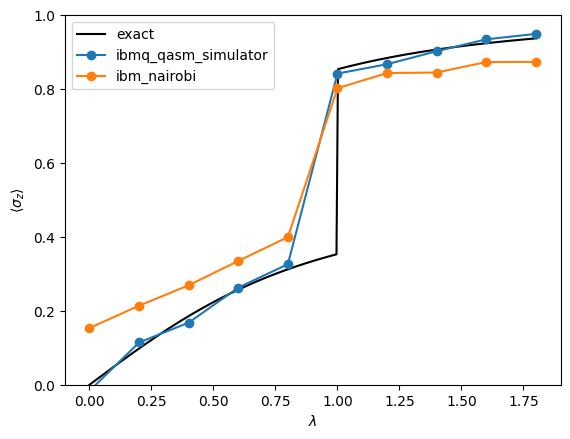
\includegraphics[width=\textwidth]{images/ground-state-magnetization}
    \caption{The expected value of the magnetization in the ground state.%
      \label{fig:ground-state-magnetization}}
  \end{figure}
  The differences on the real quantum computer are coming from the quantum noise present. The results also show an improvement over the results in Ref.~\cite{CerveraLierta18}, which fail to show a distict phase transition near \( \lambda = 1 \). This is likely due to improvements in the quantum systems over the last five years, supporting the idea that the exact Hamiltonian simulations can be used to benchmark quantum computers.

  The time evolution of the transverse magnetization are presented in Fig~\ref{fig:time-evolution-mangetization}.
  \begin{figure}
      \centering
      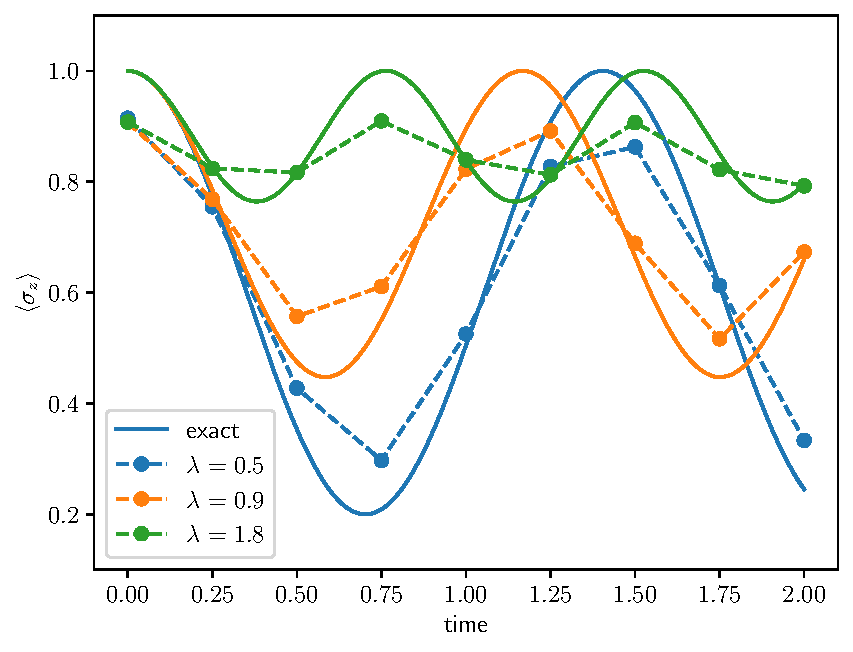
\includegraphics[width=\textwidth]{images/time-evolution-magnetization}
      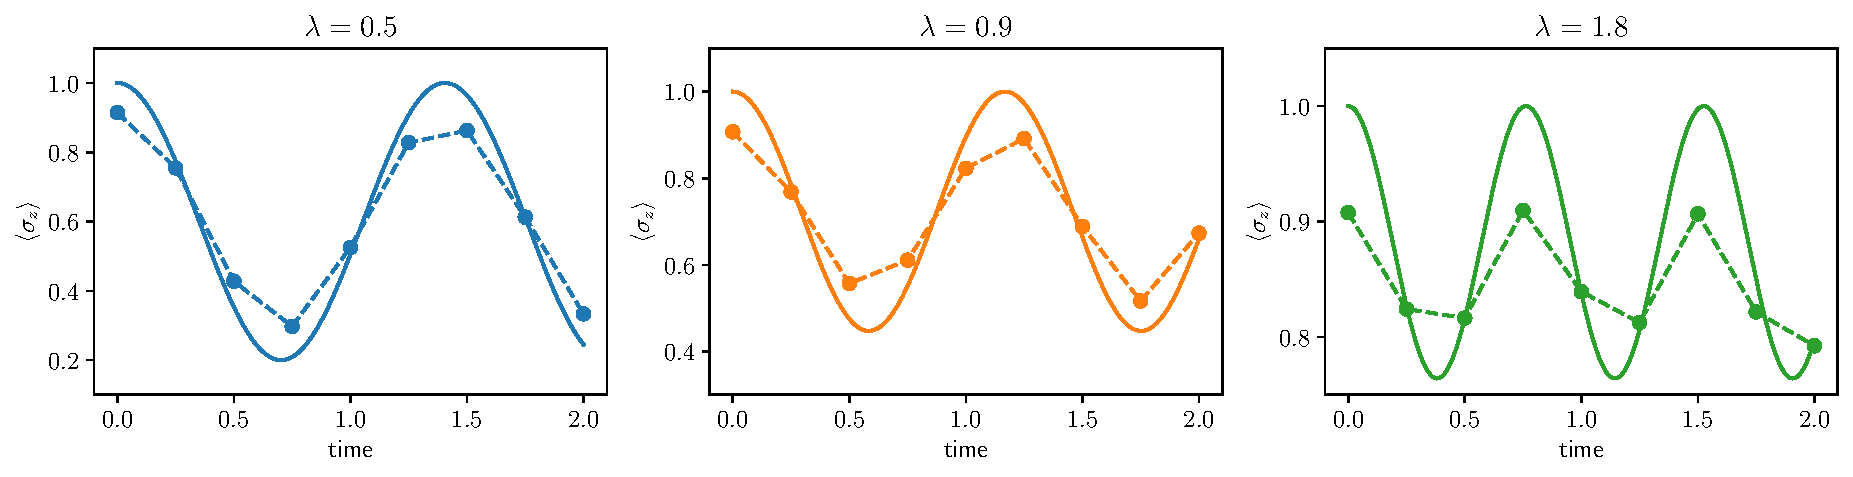
\includegraphics[width=\textwidth]
        {images/time-evolution-magnetization-separate}
      \caption{The time evolution results on \texttt{ibm\_nairobi}.%
        \label{fig:time-evolution-mangetization}}
  \end{figure}
  These results also more closely match the expected results, reaching greater magnetizations than the results in Ref.~\cite{CerveraLierta18}. The magnetization appears to consistently undershoot the expected value by about \( 0.1 \).

  \printbibliography
\end{document}
